\section{CHARM Demo}

In this section we present a web demonstration platform, accessible at \url{https://d5demos.mpi-inf.mpg.de/charm}, that showcases CHARM as a predictive model for extracting personal knowledge from conversational utterances \cite{tigunova2021exploring}. The contribution of such system is twofold. First, the demonstration can help users protect their privacy by identifying parts of their generated content that could give away personal information. Second, the system shows in detail how the model arrives at the prediction, which is rarely 
reflected in most automated extraction systems for personal facts.

\subsection{Motivation} 

Personal knowledge is a versatile resource that is valuable for a wide range of downstream applications. As observed in Chapter \ref{chap_backgr}, there has been ample research on automatically extracting or inferring personal knowledge. The developed models for conversational data predict a wide range of personal attributes from basic demographics and personality features to fine-grained interests and biography facts.

Such models can benefit many practical applications, yet they potentially endanger privacy. Thus, users should be given an opportunity to assess how the extraction models work in a transparent way. First, this enables users to explore how much personal information can be revealed from what they say online. Second, this helps to explain the reasoning leading to specific personalized ads and recommendations.

To address this issue we develop a demonstration platform for personal knowledge extraction methods, with CHARM as the underlying model. Such setting gives users a chance to directly observe the model's predictions (as opposed to, for example, trying to interpret the recommendations and ads on the websites).

We demonstrate CHARM's predictive capacity in two possible scenarios. The first setting demonstrates how a chatbot can interact with users to collect personal facts, designed as a guessing game. 
This provides the users with an opportunity to give creative answers and explore the model's capabilities, particularly in inferring the attribute values from given \emph{cues} (e.g., `\textit{pool}', `\textit{paddles}') instead of explicit \emph{mentions} (e.g., `\textit{swimming}'). 
Users can also try out some rare values (e.g., \emph{quilting}) or test how fine-grained the predictions can be (e.g., \emph{curling} instead of \emph{sports}). 
The second scenario involves applying CHARM on the real users' posts on social media. 

The proposed CHARM demonstration enables the users to \emph{(i)} see what personal information is disclosed by their answers or social media posts, and \emph{(ii)} get explanations on how the prediction was made. This supports users' privacy and model's transparency, which are rarely considered by personalized downstream applications, such as search or recommendation engines.

%The top scoring attribute values are yielded by the model as predictions.
%Explanations are given in the form of textual cues found in the input utterances, as well as retrieved web documents used to indicate the attribute values. The users can then identify revealing utterances and see how the predictions change if they modify the lexicon they use. 
%Moreover, we provide an \emph{unseen} mode  to examine how robust the model is for the values that were not seen during training.

\subsection{Demonstration platform}

\label{sec:demo}

Our demonstration system supports prediction of two personal attributes: \textit{profession} and \textit{hobby}, and incorporates two input scenarios: \emph{chatbot} and \emph{social media} settings.

\subsubsection{Input scenarios}

\paragraph{Chatbot setting.} Personal assistants enhanced with background knowledge about their users can give better responses and initiate more interesting conversations.
In this setting, we imitate how an intelligent assistant can infer personal facts from interactions with its user without asking explicit questions, such as \emph{``What is your job?''}. 
The interaction is designed as a game, where the chatbot asks several attribute-related questions, as shown in Figure~\ref{conv}.

\begin{figure}[th!]
\centering
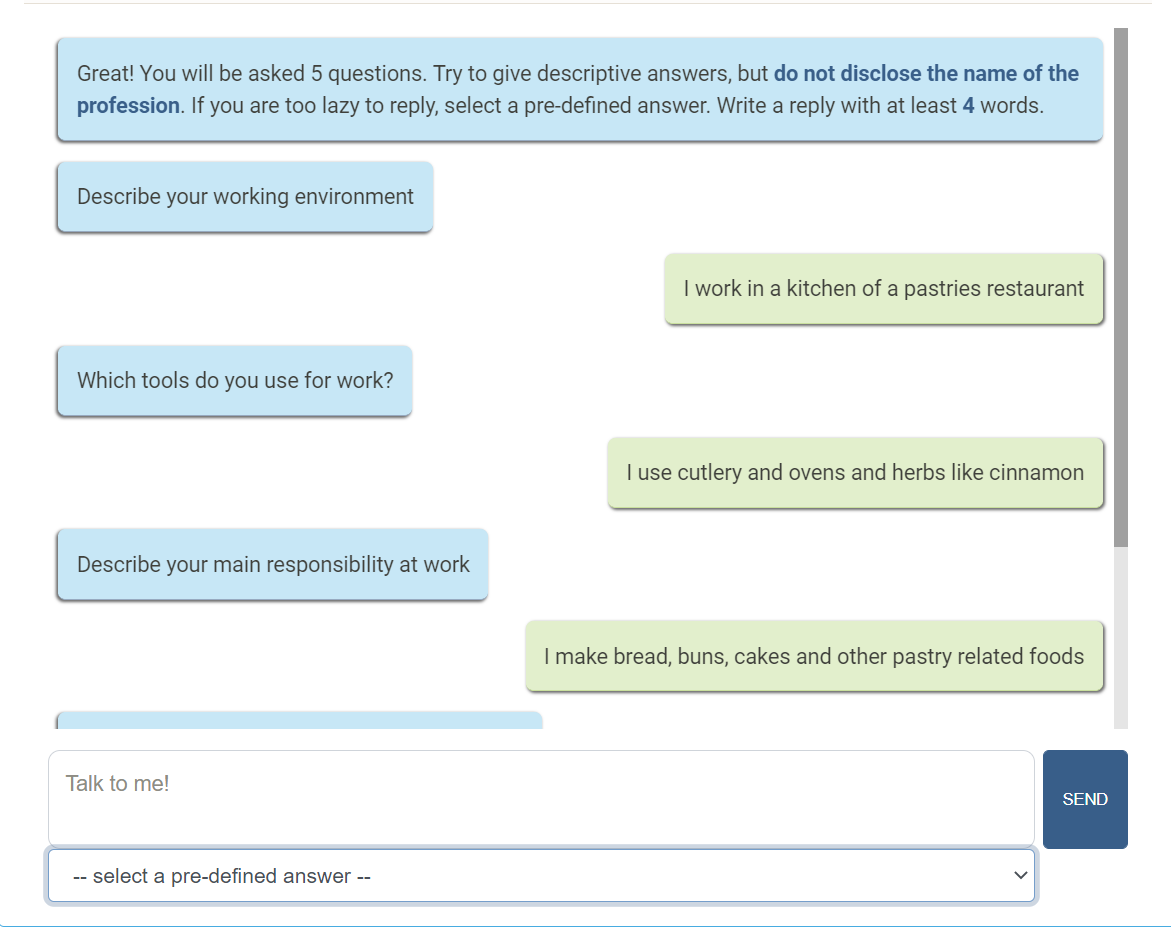
\includegraphics[width=0.85\textwidth]{imgs/conv-baker.png}
\vspace*{-0.3cm}
\caption{Chatbot conversation.}
\label{conv}
\end{figure}

Users are supposed to avoid mentioning the attribute value they have in mind, but rather to provide the chatbot with indirect cues like \emph{``I work in a \textbf{kitchen}''} for the \emph{``Describe your working environment''} question. The number of questions is fixed to 5, which should provide enough cues in the user's utterances to predict the correct attribute value without a lengthy interaction. We also require that the user's response to a question contains at least four words. 

To give users an idea of how responses should look, we provide a sample reply to each question, which the user can choose instead of typing their own responses. Each reply is designed as if it was given by a person with some pre-defined attribute value. For example, for the chat-bot request \textit{``Describe the place where you do your hobby''}, we add a predefined reply \textit{``It is a pool or open water''} related to \textit{hobby:swimming}. 

\paragraph{Social media setting.} 
Social media traces of online users are utilized by large companies for personalizing their services and ads, making them more interesting and relevant. However, the users have neither control nor understanding of how their personal information was inferred and which parts of their content revealed it. Ideally, the users should be given an opportunity to identify and exclude their posts which can potentially expose personal facts. 

In the social media scenario, we show how CHARM 
can dig through the vast amount of 
noisy 
conversational data in social media to find accurate cues for prediction.
Users can type or paste their social media posts (e.g., Reddit submissions) into the social media interface of our demonstration platform. Together with CHARM's predictions, the users will be provided with the information which parts of their utterances were used by the predictive model. It provides an opportunity to delete or modify the exposing content, and to check whether the model can still arrive at the same prediction after a partial content removal.

As in the chatbot scenario, we provide samples of synthetic user-generated content, resembling submissions in Reddit discussion threads, corresponding to pre-defined attribute values.
%that are often noisy, colloquial and unstructured.


\begin{figure}[th!]
    \centering
    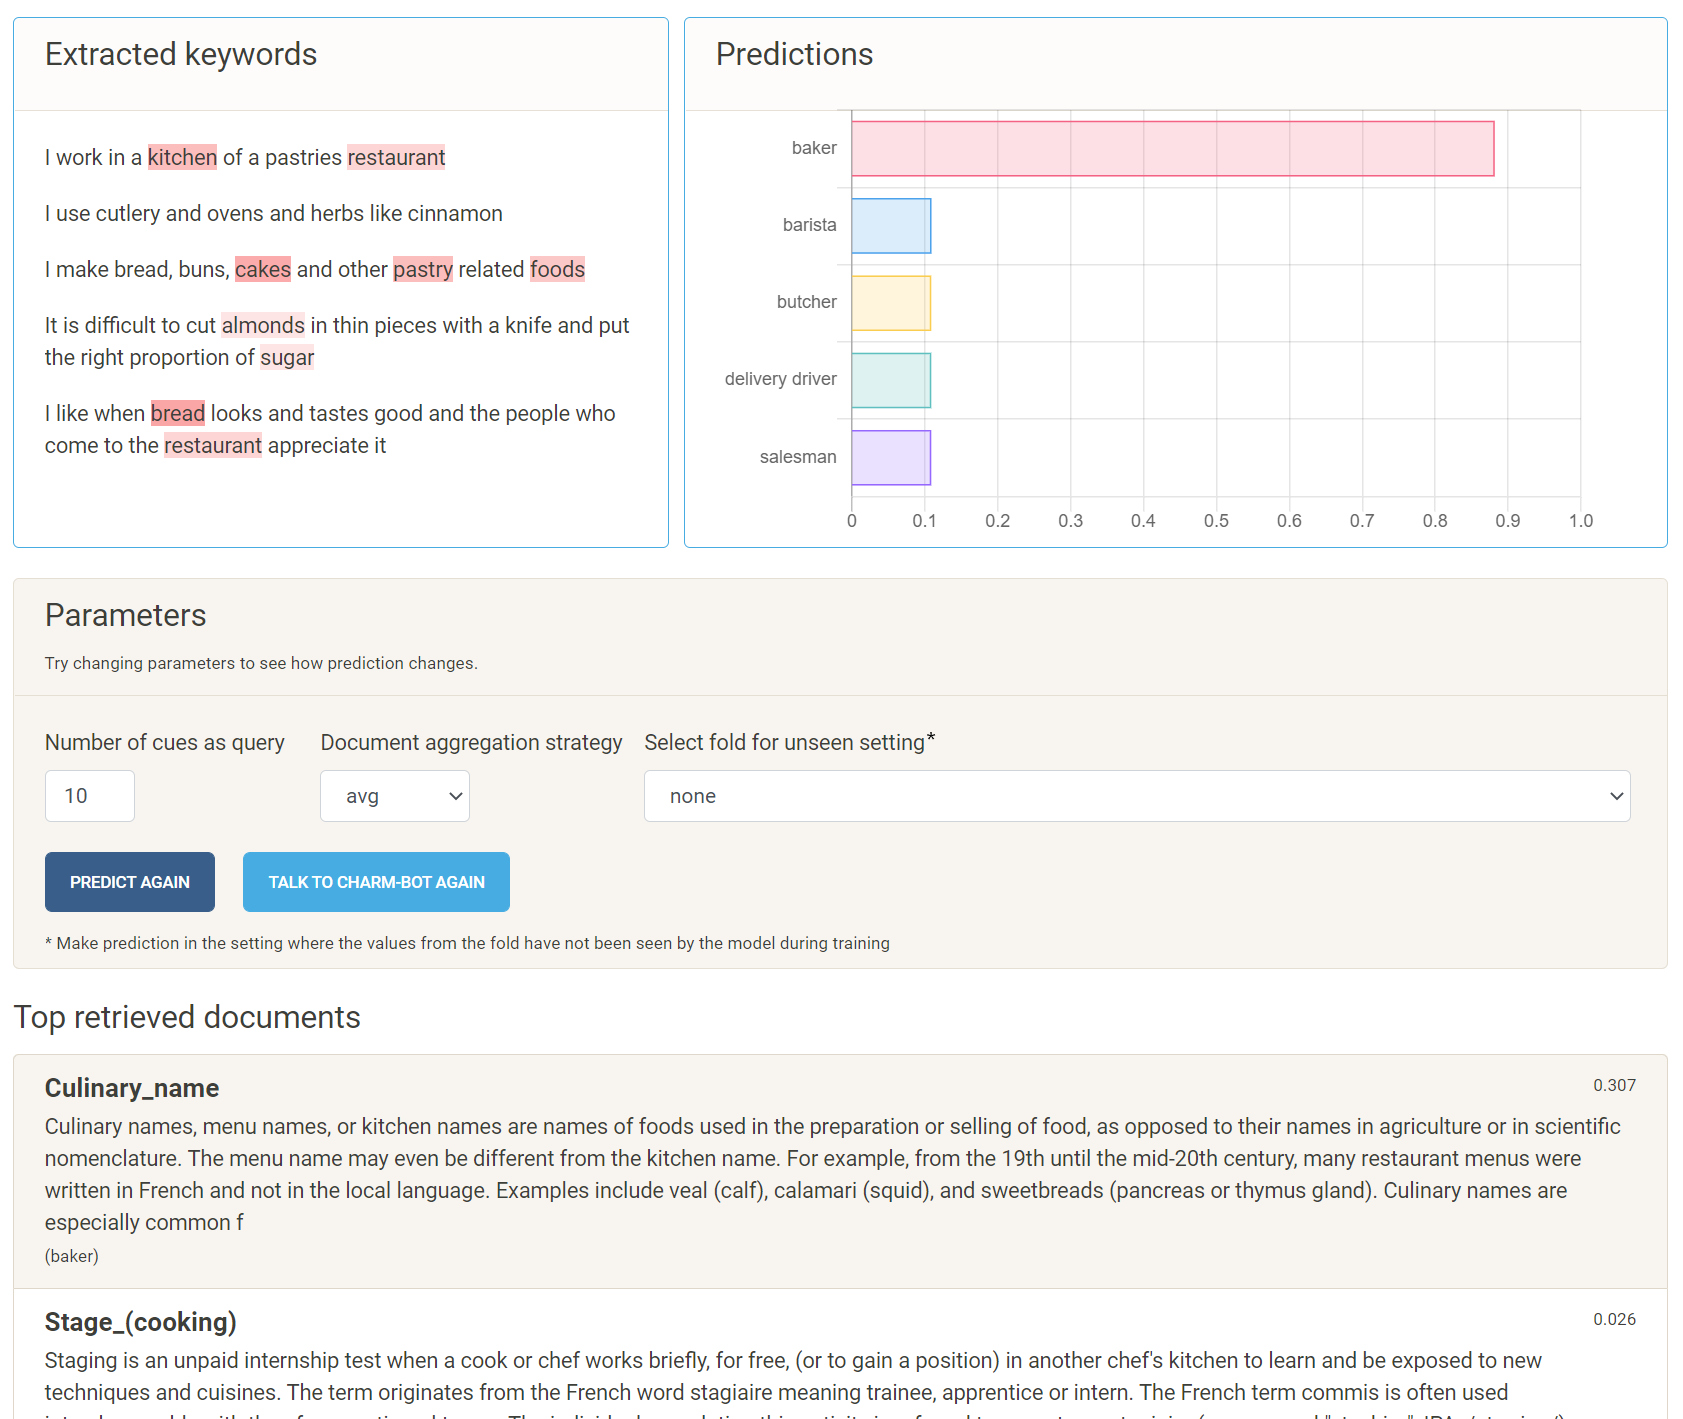
\includegraphics[width=0.95\textwidth]{imgs/prediction-baker.png}
    \caption{CHARM prediction result.}
    \label{pred_img}
\end{figure}

\subsubsection{Prediction results} 
As shown in Figure \ref{pred_img}, the prediction page presented to the user consists of intermediate results for both components of CHARM (\textit{term scoring model} and \textit{document ranker}) and the final prediction. To show the keyword selection step, we highlight the words in the user's utterances with an intensity that corresponds to the words' scores given by the {term scoring model}. The results for the document ranking step are presented as a sorted list of 10 top scoring documents. Each document is linked to the original article on the web. Finally, we show top 5 attribute value predictions after aggregating document scores. We normalized them to $[0,1]$ scale for interpretability when comparing the model's confidence in predicting each value. 

\subsubsection{Model parameters} 
The demonstration allows the users to explore how CHARM's predictions change depending on its two hyperparameters: the \emph{number of extracted keywords} and the \emph{document aggregation strategy}. 
We set the default number of extracted keywords as $\frac{1}{3}$ of the number of meaningful terms in the input utterances (after removing stopwords and digits), 
with 10 as the maximum value.
Setting the number of keywords too high can result in a noisy query and inadequate behaviour of the retrieval model. 
On the other hand, small number of keywords can be insufficient for accurate document retrieval.

As the document aggregation strategy, the user can choose between \texttt{max} and \texttt{average} functions. \texttt{Max} operation is useful when the document collection is noisy and the prediction score should come from a single most relevant document per attribute value. The \texttt{average} function is good to provide a balanced prediction based on all available documents, protecting the result from being spoilt by an inappropriate top scoring document. For this reason we selected \texttt{average} as the default aggregation function.

We selected to use \charm{KNRM} as the underlying model and \wiki{category} as document collection for our demonstration platform. As shown in the experiments described in Section \ref{charm_results}, this combination of ranker and document collection shows superior performance in most test cases. \wiki{category} is a sweet spot between simple \wiki{page}, which can only provide trivial explanations with pages matching attribute value name, and Web-search collection, which is difficult for the end-user to interpret because of noisy and ill-formatted pages. %On the other hand, \wiki{category} shows how CHARM's predictions can be determined by the topical pages from the same category.
 
\subsubsection{Unseen scenario} 
We also showcase CHARM's ability to predict attribute values
that are lacking training samples.
We train 10 variants of the model, in which each model has seen samples from only 90\% of the attribute values during training; 10\% of the attribute values are \emph{unseen}. 
In our web interface, the users can try to make a prediction using one of those models
by selecting the option where the listed attribute values are unseen. 
For example, for the input utterances \{\emph{``I was pedaling the whole evening''}, \emph{``I don't like long walks, I like spending time on my bike''}\}, it can be interesting to see the prediction result by the model not trained on hobby value \emph{cycling}. 

\subsection{Case study}
\label{sec:case-study}

In this section we present a walk-though scenario for the chatbot setting. As input we take a set of utterances from a pre-defined personality having \textit{profession}: \textit{baker}. In the first step, the chatbot asks the user 5 questions, such as \emph{``How do you start your day at work?''}. We give an excerpt of the conversation between the user and the chatbot in Figure \ref{conv}. 

On the next step the user is taken to the prediction result page, shown in Figure~\ref{pred_img}. Using the default heuristic, CHARM extracts \nolinebreak 9 keywords from the input.
The resulting query thus becomes \textit{``kitchen restaurant cakes pastry foods almonds sugar bread restaurant''}. From Figure \ref{pred_img} it can be seen that the words `\textit{cakes}', `\textit{bread}' and `\textit{pastry}' were assigned high scores by the term scoring model, whereas more general words, like `\textit{restaurant}', were included in the query but received lower scores.

The default document score aggregation strategy is \texttt{average}, which helps to overcome the influence of the top scoring document \emph{wiki:Stage\_(cooking)} (a culinary internship), which was automatically labeled as \textit{student}. 
Thus, if the user changes the aggregation function to \texttt{max}, the effect of document scoring makes \emph{baker} and \emph{student} almost equally probable. 

The qualitative results of varying the parameters of CHARM on our exemplary input are shown in Table \ref{param_change}. 
Setting the number of keywords to 2 still does not prevent CHARM from making a correct prediction using a concise query \textit{``bread ovens''}. However, the model is not robust with a long query, resulting in the ranker yielding many documents equally relevant to this query, like \emph{baker}, \emph{barista} and \emph{butcher} pages.

Finally, the user can inspect the behaviour of CHARM in the \emph{unseen} setup, when the value \emph{baker} was not present in the training data. To do that the user should select an unseen fold from the dropdown list, which contains the value \emph{baker}. As shown in Table \nolinebreak\ref{param_change}, CHARM is still capable of predicting the correct value. In contrast to the normal \textit{seen} setting, the difference in scores for correct and incorrect predictions is less.

\begin{table}[]
    \centering
\begin{adjustbox}{width=0.75\textwidth}
\begin{tabular}{ccc|cl}
\toprule
\begin{tabular}[c]{@{}c@{}}number of \\ keywords\end{tabular} & \begin{tabular}[c]{@{}c@{}}aggregation \\ strategy\end{tabular} & \begin{tabular}[c]{@{}c@{}}seen/unseen \\ setting\end{tabular} & \begin{tabular}[c]{@{}c@{}}correct \\ prediction score\end{tabular} & \begin{tabular}[c]{@{}c@{}}best incorrect \\ prediction score\end{tabular} \\ \midrule
10                                                            & avg                                                             & seen                                                           & 0.91                                                                & 0.19 (barista)                                                                      \\
\textbf{2}                                                    & avg                                                             & seen                                                           & 0.88                                                                & 0.19 (sailor)                                                                      \\
\textbf{25}                                                   & avg                                                             & seen                                                           & 0.85                                                                  & 0.85 (barista)                                                                      \\
10                                                            & \textbf{max}                                                    & seen                                                           & 0.89                                                                & 0.77 (student)                                                                       \\
10                                                            & avg                                                             & \textbf{unseen}                                                & 0.91                                                                & 0.32 (butcher) \\                      \bottomrule                                  
\end{tabular}
\end{adjustbox}
    \caption{Prediction scores based on CHARM parameters.}
    \label{param_change}
\end{table}